\chapter{Pulses analysis and tuning}

Having concluded that the closed-loop optimization protocol we tested would not significantly improve our circuits performance, we shifted our focus towards improvement and implementation of individual protocols to improve the accuracy of qubit operations.\\
In this chapter, I present the results of two additions to the \texttt{Qibocal} software. 
The first is the inclusion of an $RX90$ gate as a native gate, which can enhance the performance of protocols requiring qubit rotations of $\frac{\pi}{2}$.
The second is the implementation of the cryoscope, a routine first described in \cite{rol_time-domain_2020}, which is useful for correcting distortions in the magnetic flux pulse applied to the SQUID.

\section{RX90 calibration}
As discussed in Section \ref{sec:calibration}, it is possible to calibrate system parameters and perform fine-tuning routines to accurately determine the amplitude and frequency of the drive pulse required to transition the qubit from the $\ket{0}$ state to the $\ket{1}$ state. 
This calibration is essential for the correct implementation of single-qubit gates, such as the $R_X(\pi)$ rotation used in our setup.

However, executing more complex quantum circuits and algorithms requires the ability to perform a broader set of quantum operations. 
In gate-based quantum computing, and in particular for superconducting hardware platforms, this is achieved by composing more general unitary operations from a limited set of pre-defined, hardware-native quantum gates. 
These native gates are the elementary operations that are directly implementable and physically calibrated on the quantum processor.

The choice and quality of these native gates are extremly important as all higher-level gates will be decomposed into sequences of native gates, and any calibration errors in the latter can accumulate and propagate through a circuit, degrading the overall fidelity. 
Therefore, having a small, universal, and very well-calibrated set of native gates is essential for the reliable execution of quantum algorithms.

\subsection{\Qibolab native gates}\label{subsec:native_gates}
Native gates are those which can be directly implemented at the hardware level, in contrast to abstract logical gates, which must be transpiled into sequences of hardware supported primitives. 
In the case of \texttt{Qibolab}\footnote{At least for version 0.1 of \Qibolab}, the native gate set consists of $R_X(\pi)$ gate, calibrated be performing the Rabi experiments described in Section \ref{sec:Rabi}, the measurement gate and the virtual-Z (VZ) gate which is not implemented via a physical pulse but rather through a dynamic adjustment of the phase of subsequent control pulses. 
Additionally, the RX90 gate, corresponding to a $\frac{\pi}{2}$ rotation, is implemented by halving the amplitude of the calibrated $\pi$-pulse.
This native gate set, consisting of physically implemented $R_X(\pi)$, $R_X(\pi/2)$, and virtual Z gates, is sufficient for universal single-qubit control.

Indeed, it can be shown that any arbitrary single-qubit unitary operation $ U(\gamma, \theta, \phi) \in SU(2) $ can be expressed, up to a global phase, as a sequence of rotations around the $z$ and $x$ axes of the Bloch sphere:
\begin{equation}
U(\gamma, \theta, \phi) = R_Z(\gamma) R_X(\theta) R_Z(\phi).
\end{equation}
This decomposition ensures that all single-qubit operations can be realized using a combination of $ R_X $ and $ R_Z $ rotations. 

When a qubit is driven by a resonant microwave pulse (with detuning $ \delta = 0 $), the resulting evolution is a rotation around an axis $\hat{n} = (\cos\phi, -\sin\phi, 0)$ lying in the equatorial plane of the Bloch sphere. 
The associated unitary can be written as:
\begin{equation}
R_{\hat{n}(\phi)}(\theta) = \exp\left( -i \frac{\theta}{2} \left[ \cos(\phi)\sigma_x - \sin(\phi)\sigma_y \right] \right).
\end{equation}

This operation can be equivalently expressed through conjugation of an $R_X$ rotation by two $R_Z$ rotations:
\begin{equation}
R_{\hat{n}(\phi)}(\theta) = R_Z(-\phi) R_X(\theta) R_Z(\phi) = U(-\phi, \theta, \phi).
\end{equation}
From this, it follows that any arbitrary unitary $ U(\gamma, \theta, \phi) $ can be implemented as:
\begin{equation}
U(\gamma, \theta, \phi) = R_Z(\gamma + \phi) \cdot R_Z(-\phi) R_X(\theta) R_Z(\phi) = R_Z(\gamma + \phi) \cdot U(-\phi, \theta, \phi).
\end{equation}

Note that, in practice, this final $R_Z$ rotation does not need to be realized as a physical pulse. 
Instead, it can be implemented virtually by adjusting the phase reference of subsequent pulses, a technique known as the virtual-Z gate\cite{McKay_2017}. \\
The ability to compose any single-qubit gate using only $R_X$ and virtual-Z operations \cite{boykin1999universalfaulttolerantquantumcomputing} confirms the sufficiency of this native gate set for universal single-qubit control. For instance, even a restricted $ R_X $ rotation such as $ R_X(\pi) $, when combined with arbitrary-angle $ R_Z $ gates, forms a universal set due to the non-commuting nature of these operations.
By alternating $ R_X(\pi) $ pulses with phase-adjustable $ R_Z $ gates, one can synthesize any $SU(2)$ unitary up to global phase.

\subsection{RX90 as native gate}
Since many routines and protocols in quantum computing rely on $R_X(\pi/2)$ rotations, we decided to include the $R_X(\pi/2)$ gate in the native set of Qibolab.
The main motivation for this addition is that, until now, we had assumed the amplitude or duration of the $R_X(\pi/2)$ gate were exactly half that of the $R_X(\pi)$ pulse.
This assumption implies a perfectly linear response of the qubit to the drive pulse, an idealization which may not be satisfied in practice due to nonlinearities in the system or imperfections in the pulse generation and transmission.

To support this change I updated the \tt{native.py} module, which provides the data containers for holding the pulse parameters required for implementing every native gate.
Additionally, I modified the calibration experiments presented in Section \ref{sec:calibration} to support the calibration of this new gate.
In particular, I adapted the code used for the various implementations of the Rabi oscillation measurement protocol to include the $R_X(\pi/2)$ gate.

\subsection{Results}
In the following I will present the results obtained performing the modified version of the Rabi experiments implemented in \Qibocal.

\begin{table}[h!]
    \centering
    \begin{tabular}{c|cc|cc|cc}
        \toprule
        \textbf{Qubit} & \multicolumn{2}{c|}{\textbf{RX}} & \multicolumn{2}{c|}{\textbf{RX / 2}} & \multicolumn{2}{c|}{\textbf{RX90}} \\
         & \textbf{Amplitude} & \textbf{Errors} & \textbf{Amplitude} & \textbf{Errors} & \textbf{Amplitude} & \textbf{Errors} \\
         & \textbf{[a.u.]}  & \textbf{[a.u.]}  & \textbf{[a.u.]}  & \textbf{[a.u.]} & \textbf{[a.u.]} & \textbf{[a.u.]}\\
        \midrule
        \textbf{B1} & $8.72 \cdot 10^{-2}$ & $0.001 \cdot 10^{-2}$ & $4.36 \cdot 10^{-2}$ & $0.005 \cdot 10^{-2}$ & $3.711 \cdot 10^{-2}$ & $0.006 \cdot 10^{-2}$ \\
        \textbf{B2} & $9.433 \cdot 10^{-2}$ & $0.008 \cdot 10^{-2}$ & $4.765 \cdot 10^{-2}$ & $0.004 \cdot 10^{-2}$ & $4.047 \cdot 10^{-2}$ & $0.004 \cdot 10^{-2}$ \\
        \textbf{B3} & $1.292 \cdot 10^{-1}$ & $0.001 \cdot 10^{-1}$ & $0.646 \cdot 10^{-1}$ & $0.003 \cdot 10^{-2}$ & $6.058 \cdot 10^{-2}$ & $0.005 \cdot 10^{-2}$ \\
        \textbf{B4} & $1.517 \cdot 10^{-1}$ & $0.001 \cdot 10^{-1}$ & $0.7585 \cdot 10^{-1}$ & $0.005 \cdot 10^{-2}$ & $7.216 \cdot 10^{-2}$ & $0.005 \cdot 10^{-2}$ \\
        \bottomrule
    \end{tabular}
    \caption{Amplitude values for the $R_X(\pi)$, half $R_X(\pi)$ and $R_X(\pi/2)$ pulses as measured with the \tt{rabi\_amplitude} protocol with a fixed duration of 40 ns.}
\end{table}


\section{Flux pulse correction}

\section{Flux pulse correction}

\subsection{Cryoscope}
The protocol that I describe in this section was first introduced in \cite{rol_time-domain_2020}, the goal is to reconstruct the magnetic flux signal that bias the SQUID and then determine predistortions that needs to be applied to a flux pulse signal so that the qubit receives the flux pulse as intended by the experimenter.

As explained in section \ref{sec:cQED}, accurate dynamical control of qubit frequency is of key importance to realize single- and two-qubit gates.
One of the on-chip control variable that is used on QunatumWare chip is the magnteic flux through a SQUID loop, the signal for magnetic flux control originates from an arbitrary waveform genarator (AWG) which operates at room temperature.\\
As the signal propagates through various electrical components along the control line leading to the quantum device it undergoes linear dynamical distortions. 
If not properly compensated, these distortions can degrade gate performance, impacting experiments fidelity and repeatability.\\

In \cite{rol_time-domain_2020} is proposed a technique to characterize flux-pulse distortions induced by components inside the dilution refrigerator by directly measuring the qubit state.
In this routine we send the qubit a pulse sequence where a flux pulse of varying duration $\tau$ is embedded between two $\frac{\pi}{2}$ pulses which are always separated by a fixed interval $T_{sep}$.\\
The first $\frac{\pi}{2}$ pulse rotates the qubit of $\frac{\pi}{2}$ around the $y$ axis of the Bloch sphere changing its state from $\ket{0}$ to $\frac{\ket{0}+\ket{1}}{\sqrt{2}}$.

When a flux pulse $\Phi_{Q,\tau}(t)$ of duration $\tau$ is sent to the qubit\footnote{To send a $\Phi_{Q,\tau}(t)$ flux pulse we are actually sending a $V_{\text{in},\tau}(t)$ DAC pulse} after the first $\frac{\pi}{2}$ pulse, the qubits evolve to the state $\frac{\ket{0}+e^{i\varphi_\tau}\ket{1}}{\sqrt{2}}$ with relative quantum phase 
\begin{equation}\label{eq:phi}
    \frac{\varphi_{\tau}}{2\pi} = \int_{0}^{T_{sep}} \Delta f_Q (\Phi_{Q,\tau(t)})\text{d}t = \int_{0}^{\tau} \Delta f_Q (\Phi_{Q,\tau(t)})\text{d}t + \int_{\tau}^{T_{sep}} \Delta f_Q (\Phi_{Q,\tau(t)})\text{d}t
\end{equation}
where in the second step we separated the contributions from flux response up to $\tau$ and the turn-off transient \footnote{In \hyperref[app:AppendixB]{Appendix B} I calculate the relative phase $\varphi_{\tau}$ for a more general shape of the flux pulse.}. 

The experiment is then completed with a $\frac{\pi}{2}$ rotation aroud the $y$- or $x$-axis of the Bloch sphere to measure respectively the $\langle X \rangle$ or $\langle Y \rangle$ components of the Bloch vector when applying the measurement gate $MZ$. 
From the measurement of $\langle X \rangle$ and $\langle Y \rangle$ we can extract the relative phase $\phi_{\tau}$.\\

Then we can estimate $\Phi_Q(t)$ in the interval $[\tau,\tau+\Delta\tau]$ as follows. From the measurement of $\phi_{\tau + \Delta\tau}$ and $\phi_\tau$ we can compute $\overline{\Delta f_R}$:
\begin{align}\label{eq:detuning}
    \overline{\Delta f_R} &= \frac{\phi_{\tau+\Delta\tau} - \phi_\tau}{2\pi\Delta\tau}\\ 
    &= \frac{1}{\Delta\tau}\left(\int_{0}^{\tau+\Delta\tau}\Delta f_Q (\Phi_{Q,\tau+\Delta\tau}(t))dt + \int_{\tau+\Delta\tau}^{T_{sep}}\Delta f_Q (\Phi_{Q,\tau+\Delta\tau}(t))dt\right) \\
    &-\frac{1}{\Delta\tau}\left(\int_{0}^{\tau}\Delta f_Q (\Phi_{Q,\tau}(t))dt - \int_{\tau}^{T_{sep}}\Delta f_Q (\Phi_{Q,\tau}(t))dt\right)\\
    &=\frac{1}{\Delta\tau}\left(\int_{\tau}^{\tau+\Delta\tau} \Delta f_Q(\Phi_{Q,\tau+\Delta\tau})dt + \int_{\tau+\Delta\tau}^{T_{sep}}\Delta f_Q (\Phi_{Q,\tau+\Delta\tau}(t))dt - \int_{\tau}^{T_{sep}}\Delta f_Q (\Phi_{Q,\tau}(t))dt\right)\\
    &= \frac{1}{\Delta\tau}\int_{\tau}^{\tau+\Delta\tau} \Delta f_Q(\Phi_{Q,\tau+\Delta\tau})dt + \varepsilon
\end{align}  
with \[\varepsilon = \frac{1}{\Delta\tau}\left(\int_{\tau+\Delta\tau}^{T_{sep}}\Delta f_Q (\Phi_{Q,\tau+\Delta\tau}(t))dt - \int_{\tau}^{T_{sep}}\Delta f_Q (\Phi_{Q,\tau}(t))dt\right)\]
The phase contribution from the turn-off transients is minimal due to the sharp return to the first-order flux-insensitive sweet spot of the nearly quadratic $\Delta f_Q(\Phi_Q)$; 
numerical simulations suggest that $|\varepsilon|/\Delta f_R$ remains within the range of approximately $10^{-2}$ to $10^{-3}$ for typical dynamical distortions in commonly used electronic components \cite{negligible} \cite{Langford2017}, for this reason it will be neglected.\\

Then we can obtain the reconstructed flux pulse $\Phi_R(t)$ inverting eq. \ref{eq:freqdepndenceonflux}.

In the following sections I will describe how we used this protocol to reconstruct the voltage to flux step response, and then how to determine and apply pre-distortions corrections to the control waveforms.

\subsubsection{Pulse reconstruction}
La prima cosa è la costruzione della seuqneza di impulsi che devono essere mandati al qubit.
Come descritto nella sezione precedente il protocollo per la ricostruzione dell'impulso di flusso è un esperimento Ramsey-like in cui embedded tra i due microwave pulses, separated by a constant time $T_{sep}$ a flux pulse of varying duration $\tau$.
Nel nostro caso abbiamo deciso di fissare $T_{sep}$ pari a $100$ ns oltre la durata dell'impulso di flusso più lungo to negate the need for fine timing calibration, as suggested in \cite{rol_time-domain_2020}, mentre lo step $\Delta\tau$ con cui viene variata la durata dell'impulso di flusso è stabilita dall'utente.
Nello specifico, the user può, tramite runcard \footnote{In qibocal tutte i protocolli vengono deployati tramite runcard scritta in YAML con cui l'utente può fissare i parametri relativi all'esperimento che vuole eseguire} fissare i valori per la durata minima (\tt{duration\_min}) e massima (\tt{duration\_max}) dell'impulso di flusso e lo step con cui variare la durata dell'impulso (\tt{duration\_step}) coincidente con l'intervallo $\Delta\tau$ in Equation \ref{eq:detuning}.

The flux pulse amplitude can also be set by the user tramite il parametro \tt{flux\_pulse amplitude} ma è consigliabile utilizzare una ampiezza che induca nel qubit un detuning dallo sweetspot che sia vicino a quello necessario nella maggior parte dei casi in cui utilizzo l'impulso di flusso.
Negli esempi presentati nel seguito the flux pulse amplitude è stata scelta in modo tale da indurre un detuning di circa 1 GHz che è quella che viene utilizzata nella maggior parte delle applicazioni \cite{Langford2017}, \cite{Bultink_2020}, \cite{Rol2019iju}.

Dopo aver costruito la pulse sequence, sia quella che si conclude con $R_X(\pi/2)$ per misurare $\langle Y \rangle$ e $R_Y(\pi/2)$ per misurare $\langle X \rangle$, questi dati vengono combinato per ottenere $\phi_\tau$
\begin{comment}
    *come otteniamo la fase
    * come processiamo la fase
    * savgol filter + discussione dei parametr
\end{comment}

In the following sections I will describe how we used this protocol to reconstruct the voltage to flux step response, and then how to determine and apply pre-distortions corrections to the control waveforms.

\subsubsection{Pulse reconstruction}
La prima cosa è la costruzione della seuqneza di impulsi che devono essere mandati al qubit.
Come descritto nella sezione precedente il protocollo per la ricostruzione dell'impulso di flusso è un esperimento Ramsey-like in cui embedded tra i due microwave pulses, separated by a constant time $T_{sep}$ a flux pulse of varying duration $\tau$.
Nel nostro caso abbiamo deciso di fissare $T_{sep}$ pari a $100$ ns oltre la durata dell'impulso di flusso più lungo to negate the need for fine timing calibration, as suggested in \cite{rol_time-domain_2020}, mentre lo step $\Delta\tau$ con cui viene variata la durata dell'impulso di flusso è stabilita dall'utente.
Nello specifico, the user può, tramite runcard \footnote{In qibocal tutte i protocolli vengono deployati tramite runcard scritta in YAML con cui l'utente può fissare i parametri relativi all'esperimento che vuole eseguire} fissare i valori per la durata minima (\tt{duration\_min}) e massima (\tt{duration\_max}) dell'impulso di flusso e lo step con cui variare la durata dell'impulso (\tt{duration\_step}) coincidente con l'intervallo $\Delta\tau$ in Equation \ref{eq:detuning}.

The flux pulse amplitude can also be set by the user tramite il parametro \tt{flux\_pulse amplitude} ma è consigliabile utilizzare una ampiezza che induca nel qubit un detuning dallo sweetspot che sia vicino a quello necessario nella maggior parte dei casi in cui utilizzo l'impulso di flusso.
Negli esempi presentati nel seguito the flux pulse amplitude è stata scelta in modo tale da indurre un detuning di circa 1 GHz che è quella che viene utilizzata nella maggior parte delle applicazioni \cite{Langford2017}, \cite{Bultink_2020}, \cite{Rol2019iju}.

Dopo aver costruito la pulse sequence, sia quella che si conclude con $R_X(\pi/2)$ per misurare $\langle Y \rangle$ e $R_Y(\pi/2)$ per misurare $\langle X \rangle$, questi dati vengono combinato per ottenere $\phi_\tau$
\begin{comment}
    *come otteniamo la fase
    * come processiamo la fase
    * savgol filter + discussione dei parametr
\end{comment}

%TODO: provare ad aggiungere più correzioni esponenziali

\subsection{Filter determination}
Our final goal is to predistort the waveforms digitally using finite- and infinite impulse response filters applied in real time.

\subsubsection{IIR corrections}
\subsubsection{FIR corrections}
Una volta trovati i feedback e feedforward taps per gli IIR filters, è necessario trovare gli FIR per correggere il segnale su scale di tempo più brevi. 

for description and notes on \tt{CMA-ES} see section \ref{Sec:OptimizationMethods}

\subsubsection{Output filters in QM}

%Spiegare come applica i filtri quantum machines
Each analog output port of the OPX system used in this work is equipped with a digital filter that is applied to the signal in the digital domain before conversion to analog. The filters are provided to the OPX via the \texttt{parameters.json} file, which contains the coefficients for the feedforward and feedback components according to the equation
\begin{equation}\label{eq:OPX_filter}
    y[n] = \sum_{m=1}^{M} a_m y[n - m] + \sum_{k=0}^{K} b_k x[n - k],
\end{equation}
where $y[n]$ is the output signal, $x[n]$ is the input waveform, $a_m$ are the feedback coefficients, and $b_k$ are the feedforward coefficients.

In our case, we have a set of feedback coefficients determined through IIR correction and two sets of feedforward coefficients: the first obtained from the IIR-based correction, and the second from FIR-based correction on short timescales. 
To uniquely determine the coefficients to be passed to the electronics, it is necessary to derive a single set of feedforward coefficients and a single set of feedback coefficients by combining the two sets of feedforward filters through convolution.

Infatti posso considerare il segnale di input $x$ a cui applico un primo filtro IIR ottenendo così un segnale in output $y$ tale che
\begin{equation}\label{eq:y_signal}
    y[n] = \sum_{m=1}^{M} a[m]y[n-m] + \sum_{k=0}^{N} b[k] x[n-k].
\end{equation}

al segnale $y$ applico un secondo filtro IIR ottonendo quindi un segnale $z$ in output con la sgeuente forma 
\begin{equation}\label{eq:z_signal}
    z[n] = \sum_{m=1}^{M} a'[m]z[n-m] + \sum_{k=0}^{N} b'[k] y[n-k].
\end{equation}

Now I consider equation \ref{eq:y_signal} and rewrite it as
\begin{equation}\label{eq:y_signal1}
    y[n] - \sum_{m=1}^{M} a[m]y[n-m] = \sum_{k=0}^{N} b[k] x[n-k],
\end{equation} 
then by applying a Z-transform we obtain
\begin{equation}\label{eq:y_signal_transform}
    Y(z)\left(1 - \sum_{m=1}^{M} a[m] z^{-m} \right) = X(z) \left( \sum_{k=0}^{N} b[k] z^{-k} \right)
\end{equation}
so that 
\begin{align}
    H_1(z) &= \frac{Y(z)}{X(z)} = \frac{\sum_{k=0}^{N} b[k] z^{-k}}{1 - \sum_{m=1}^{M} a[m] z^{-m}} = \frac{B(z)}{A(z)} \\
    & \rightarrow Y(z) = H_1(z)X(z) = \frac{B(z)}{A(z)}X(z) \\ \label{eq:transfer1}
\end{align}

We can do the same also for equation \ref{eq:z_signal} and rewrite it as 
\begin{equation}\label{eq:z_signal1}
    z[n] = \sum_{m=1}^{M} a'[m]z[n-m] + \sum_{k=0}^{N} b'[k] y[n-k],
\end{equation}
which, by applying the Z-transform becomes
\begin{equation}\label{eq:z_signal_transform}
    Z(z)\left(1 - \sum_{m=1}^{M} a'[m] z^{-m} \right) = Y(z) \left( \sum_{k=0}^{N} b'[k] z^{-k} \right).
\end{equation}
Again we can write the the transfer function
\begin{align}
    &H_2(z) = \frac{Z(z)}{Y(z)} = \frac{\sum_{k=0}^{N} b'[k] z^{-k}}{1 - \sum_{m=1}^{M} a'[m] z^{-m}} = \frac{B'(z)}{A'(z)} \\
    \rightarrow Z(z) &= H_2(z)Y(z) = \frac{B'(z)}{A'(z)}Y(z) = \frac{B'(z)}{A'(z)} \frac{B(z)}{A(z)} X(z)\\ \label{eq:transfer2}
    &= \left( \frac{\sum_{k=0}^{N} b'[k] z^{-k}}{1 - \sum_{m=1}^{M'} a'[m] z^{-m}} \right) \left( \frac{\sum_{k=0}^{N} b[k] z^{-k}}{1 - \sum_{m=1}^{M} a[m] z^{-m}} \right) X(z)\\
\end{align}
From the transfer function we can obtain the expression for $Z(z)$ in terms of $X(z)$ 
\begin{align}
    & \rightarrow Z(z) \left(1 - \sum_{m=1}^{M} a'[m] z^{-m} \right) \left(1 - \sum_{m=1}^{M} a[m] z^{-m} \right) = \left( \sum_{k=0}^{N} b'[k] z^{-k} \right) \left( \sum_{k=0}^{N} b[k] z^{-k} \right) X(z) \\
    & \rightarrow Z(z) \left( \sum_{m=0}^{M} a'[m] z^{-m} \right) \left( \sum_{m=0}^{M} a[m] z^{-m} \right) = \left( \sum_{k=0}^{N} b'[k] z^{-k} \right) \left( \sum_{k=0}^{N} b[k] z^{-k} \right) X(z)\\ \label{eq:Zz}
\end{align}
where in the last step  ho assorbito l'1 in the sum come coeffiente $a_0$. By expanding the products we obtain
\begin{align}
    & \left( \sum_{m=0}^{M} a'[m] \right) \left( \sum_{m=0}^{M} a[m] \right) = \sum_{m=0}^{2M}\sum_{i=0}^{m} a'[i] a[m - i] = c[k], \quad\quad \text{with}\quad m = 0, \dots, 2M,\\ \label{eq:ck}
    & \left( \sum_{k=0}^{N} b'[k] \right) \left( \sum_{k=0}^{N} b[k] \right) = \sum_{k=0}^{2N} \sum_{i=0}^{k} b[i] b[k-i] = d[k], \quad\quad \text{with}\quad k = 0, \dots, 2N.\\ \label{eq:dk}
\end{align}
%so that
%\begin{align}
%    & \left( \sum_{m=0}^{M} a'[m] z^{-m} \right) \left( \sum_{m=0}^{M} a[m] z^{-m} \right) = \sum_{m=0}^{2M} c[m]z^{-m} = \sum_{m=0}^{2M}\sum_{i=0}^{m} a'[i]a[m - i]z^{-m}\\
%    & \left( \sum_{k=0}^{N} b'[k] z^{-k} \right) \left( \sum_{k=0}^{N} b[k] z^{-k} \right) = \sum_{k=0}^{2N} d[k]z^{-k} = \sum_{k=0}^{2N}\sum_{i=0}^{k} b'[k]b[k-i]z^{-k}.\\
%\end{align}

It is then possible to re-write equation \ref{eq:Zz} using the new expression for the filters
\begin{align}
    & Z(z)\left( \sum_{m=0}^{2M} c[m]z^{-m} \right) = \left( \sum_{k}^{2N} d[k]z^{-k} \right)X(z)\\
    & \rightarrow Z(z)\left(1 - \sum_{m=1}^{2M} c[m]z^{-m} \right) = \left( \sum_{k}^{2N} d[k]z^{-k} \right)X(z)\\ \label{eq:z_final}
\end{align} 

then we apply the inverse-Z-transform and obtain
\begin{align}
    & z[n] - \sum_{m=1}^{2M} c[m]z[n-m] = \sum_{k=0}^{2N} d[k] x[n-k]\\
    & z[n] = \sum_{m=1}^{2M} c[m]z[n-m] + \sum_{k=0}^{2N} d[k] x[n-k]\\
\end{align}
where the feedforward (feedback) taps of the final filters, are given by the convolution of the feedforward (feedback) taps of the two filters as shown in equations \ref{eq:ck} and \ref{eq:dk}.

\subsection{Results}

The experiments in which the impact of flux signal distortions are ones where we expect to see a clear chevron pattern, deviation from the ideal chevron pattern often indicano presenza di distorsioni nel segnale di flusso \cite{Langford2017}.

Un esempio di tale esperimento è quello che in \Qibocal è identificato come chevron, clearly the name originates from the characteristic chevron-shaped interference pattern that is expected as output of the routine.
This calibration routine is used to characterize and tune native two-qubit gates, such as the CNOT or iSWAP, which are typically implemented using sequences of flux pulses, potentially applied to multiple qubits, combined with virtual $Z$-rotations.

CNOT and iSWAP are two entangling gates: the CNOT gate flips the state of a target qubit conditional on the control qubit being in state $\ket{1}$ while the iSWAP gate exchanges the quantum states $\ket{10}\leftrightarrow\ket{01}$ introducing a phase of $i$.

For example, we can consider the pulse sequence used to calibrate the iSWAP gate between a pair of qubits consists of a $\pi$ pulse followed by a flux pulse of varying amplitude and duration, applied to the qubit with the highest frequency in the pair. 
The initial $\pi$ pulse brings the qubit into the state $\ket{1}$, while the flux pulse detunes its frequency near resonance with the second qubit. 

The iSWAP gate exploits the coherent exchange of excitations between two capacitively coupled qubits by tuning them into resonance via a flux pulse. 
When brought into resonance, the computational basis states $\ket{10}$ and $\ket{01}$ become energetically near-degenerate and interact via the coupling, resulting in a level repulsion charachteristic of an avoided crossing.
In this regime the population oscillates between the two states with a frequency determined by the coupling strength $g$; the expected population oscillation pattern follows:
\begin{equation}
    p_e(t, \Delta) = \frac{\Delta^2}{\Delta^2 + 4g^2} + \frac{4g^2}{\Delta^2 + 4g^2} \cos^2\left(\frac{\sqrt{\Delta^2 + 4g^2}}{2}t\right)
\end{equation}
where $\Delta = \omega_1 - \omega_2$, and $g$ is the coupling constant for the two qubits. This probability distribution descrive esattamente quello che in letteratura è noto come chevron pattern.
In \Qibocal la routine è utilizzata per calibrare two qubits gate perchè per esempio, By adjusting the duration $t$ of the flux pulse such that $t=\pi/2g$, the system performs a full excitation exchange, implementing an iSWAP gate up to local phase corrections.
Se anzichè calibrare l'iSWAP volessimo calibrare una CZ the pulse sequence will be the same except for the addition of an initial $\pi$ pulse applied to the qubit with the lower frequency so that both qubits are initially prepared in the $\ket{1}$ state.

The ideal chevron pattern is shown Figure \ref{fig:expected_chevron}.

\begin{figure}[h!]
    \centering
    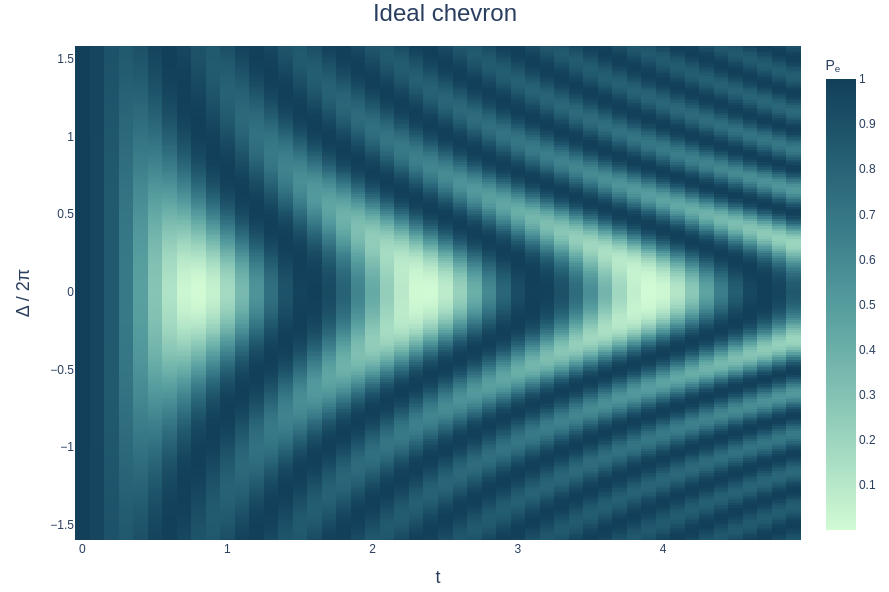
\includegraphics[width=0.45\textwidth]{figures/png/IdealChevron.png}
    \caption{Ideal chevron pattern.}
    \label{fig:expected_chevron}
\end{figure}

In Figure \ref{fig:B1B3_nofilter} and Figure \ref{fig:B2B4_nofilter}I show the actual chevron pattern obtained from the calibration of a CZ gate on our hardware without applying any digital filter.

\begin{figure}[h!]
    \centering
    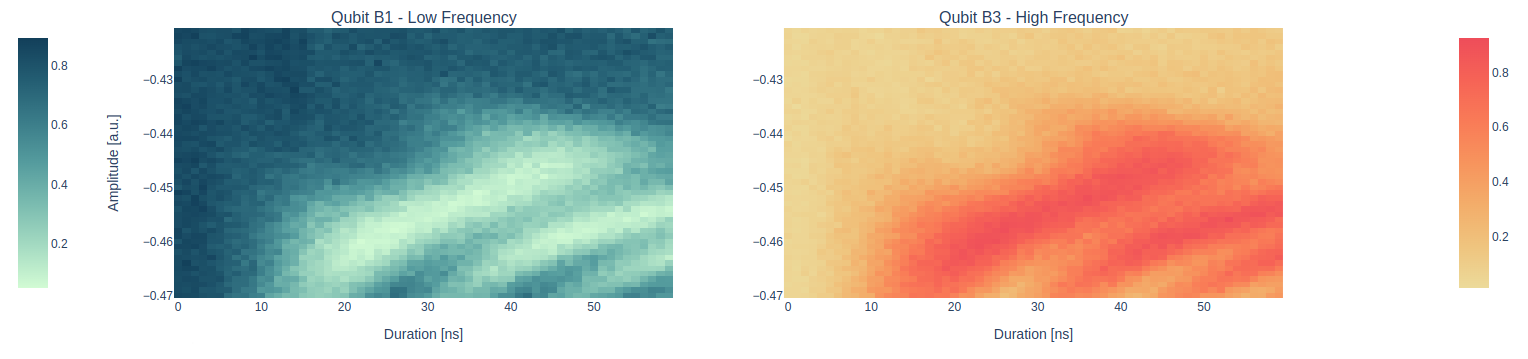
\includegraphics[width=1.15\textwidth]{figures/png/Cryoscope/B1B3_nofilter.png}
    \caption{Chevron pattern obtained from the calibration of a CZ gate on qubits \tt{B1} and \tt{B3}.\\ No filters applied.}
    \label{fig:B1B3_nofilter}
\end{figure}

\begin{figure}[h!]
    \centering
    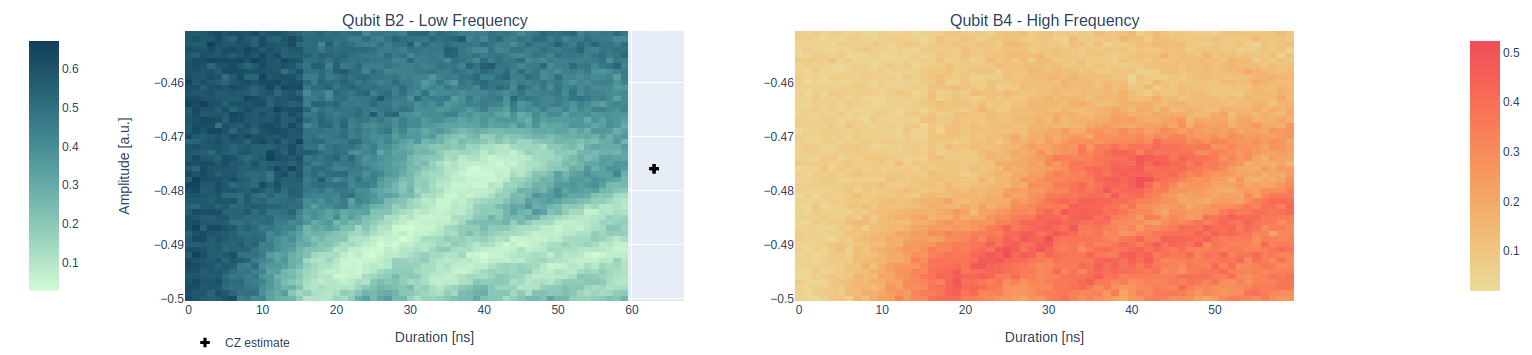
\includegraphics[width=1.15\textwidth]{figures/png/Cryoscope/B2B4_nofilter.png}
    \caption{Chevron pattern obtained from the calibration of a CZ gate on qubits \tt{B2} and \tt{B4}.\\ No filters applied.}
    \label{fig:B2B4_nofilter}
\end{figure}

After the application of the filters determined by using the cryoscope protocol the chevron pattern that we obtained is shown in Figure \ref{fig:B1B3} and Figure \ref{fig:B2B4}.

\begin{figure}[h!]
    \centering
    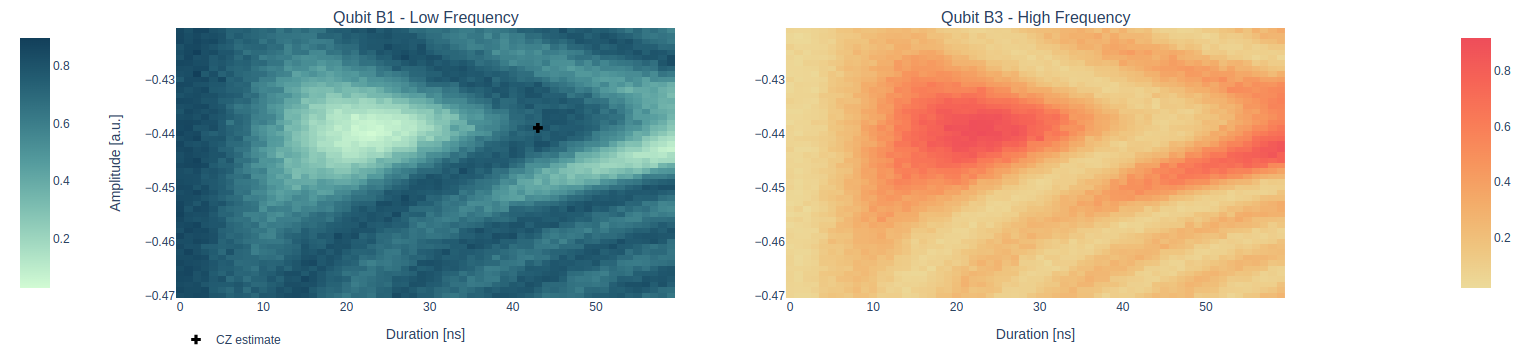
\includegraphics[width=1.15\textwidth]{figures/png/Cryoscope/B1B3.png}
    \caption{Chevron pattern obtained from the calibration of a CZ gate on qubits \tt{B1} and \tt{B3}.}
    \label{fig:B1B3}
\end{figure}

\begin{figure}[h!]
    \centering
    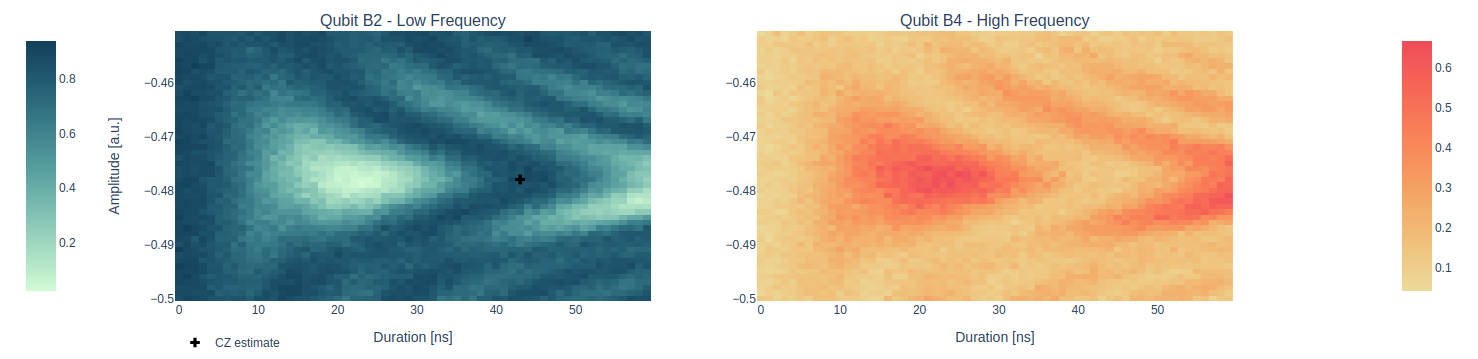
\includegraphics[width=1.15\textwidth]{figures/png/Cryoscope/B2B4.png}
    \caption{Chevron pattern obtained from the calibration of a CZ gate on qubits \tt{B2} and \tt{B4}.}
    \label{fig:B2B4}
\end{figure}
